\section{Competitive performance, recurring retention differences}\label{sec:comparisons}

In this section, we study task performance and forgetting across PEFT methods and ask whether closer geometric preservation leads to better adaptation--retention trade-offs. We also examine method-specific patterns across settings. 

\subsection{Language models: competitive performance, different retention}
We first examine whether comparable task performance in mathematics and coding is accompanied by comparable retention of general language modeling. We consider both development-selected test results and the mathematics performance--retention frontiers across learning rates and capacities.

\begin{table}[t]
\caption{Development-selected LLM test scores (\%) and FineWiki forgetting ($10^3\Delta\mathrm{NLL}$). Budgets are approximately matched: S/M/L for GSM8K; one for CodeFeedback. HE+ denotes HumanEval+. Base is one unadapted evaluation. Shading marks each column\textquotesingle s best adapted mean, including ties.}
\label{tab:math-test}\label{tab:coding-test}
\begin{center}
\textbf{(a) Mathematics: GSM8K test accuracy (\%, $\uparrow$)}\par\smallskip
\setlength{\tabcolsep}{5.9pt}\begin{tabular*}{\linewidth}{@{\extracolsep{\fill}}lcccccc}\toprule
& \multicolumn{3}{c}{Qwen2.5-7B} & \multicolumn{3}{c}{Llama-3.1-8B} \\ \cmidrule(lr){2-4}\cmidrule(l){5-7} Method & S & M & L & S & M & L \\ \midrule
\textcolor{LoRAColor}{LoRA} & $\result{math_grid_qwen_lora_7_0p001_test_mean}_{\pm\result{math_grid_qwen_lora_7_0p001_test_sd}}$ & $\result{math_grid_qwen_lora_14_1em05_test_mean}_{\pm\result{math_grid_qwen_lora_14_1em05_test_sd}}$ & $\result{math_grid_qwen_lora_28_3em05_test_mean}_{\pm\result{math_grid_qwen_lora_28_3em05_test_sd}}$ & $\result{math_grid_llama_lora_7_0p0003_test_mean}_{\pm\result{math_grid_llama_lora_7_0p0003_test_sd}}$ & \bestcell{LoRAColor}{$\bestmean{\result{math_grid_llama_lora_15_0p0003_test_mean}}_{\pm\result{math_grid_llama_lora_15_0p0003_test_sd}}$} & $\result{math_grid_llama_lora_30_0p0003_test_mean}_{\pm\result{math_grid_llama_lora_30_0p0003_test_sd}}$ \\
\textcolor{OFTColor}{OFT} & $\result{math_grid_qwen_oft_32_0p0003_test_mean}_{\pm\result{math_grid_qwen_oft_32_0p0003_test_sd}}$ & $\result{math_grid_qwen_oft_64_0p0003_test_mean}_{\pm\result{math_grid_qwen_oft_64_0p0003_test_sd}}$ & $\result{math_grid_qwen_oft_128_0p0001_test_mean}_{\pm\result{math_grid_qwen_oft_128_0p0001_test_sd}}$ & \bestcell{OFTColor}{$\bestmean{\result{math_grid_llama_oft_32_0p0003_test_mean}}_{\pm\result{math_grid_llama_oft_32_0p0003_test_sd}}$} & $\result{math_grid_llama_oft_64_0p0003_test_mean}_{\pm\result{math_grid_llama_oft_64_0p0003_test_sd}}$ & $\result{math_grid_llama_oft_128_0p0001_test_mean}_{\pm\result{math_grid_llama_oft_128_0p0001_test_sd}}$ \\
\textcolor{DoRAColor}{DoRA} & $\result{math_grid_qwen_dora_7_0p0003_test_mean}_{\pm\result{math_grid_qwen_dora_7_0p0003_test_sd}}$ & $\result{math_grid_qwen_dora_14_0p0003_test_mean}_{\pm\result{math_grid_qwen_dora_14_0p0003_test_sd}}$ & $\result{math_grid_qwen_dora_28_0p0001_test_mean}_{\pm\result{math_grid_qwen_dora_28_0p0001_test_sd}}$ & $\result{math_grid_llama_dora_7_0p0003_test_mean}_{\pm\result{math_grid_llama_dora_7_0p0003_test_sd}}$ & $\result{math_grid_llama_dora_15_0p0003_test_mean}_{\pm\result{math_grid_llama_dora_15_0p0003_test_sd}}$ & \bestcell{DoRAColor}{$\bestmean{\result{math_grid_llama_dora_30_0p0003_test_mean}}_{\pm\result{math_grid_llama_dora_30_0p0003_test_sd}}$} \\
\textcolor{PiSSAColor}{PiSSA} & \bestcell{PiSSAColor}{$\bestmean{\result{math_grid_qwen_pissa_7_3em05_test_mean}}_{\pm\result{math_grid_qwen_pissa_7_3em05_test_sd}}$} & \bestcell{PiSSAColor}{$\bestmean{\result{math_grid_qwen_pissa_14_3em05_test_mean}}_{\pm\result{math_grid_qwen_pissa_14_3em05_test_sd}}$} & $\result{math_grid_qwen_pissa_28_3em05_test_mean}_{\pm\result{math_grid_qwen_pissa_28_3em05_test_sd}}$ & $\result{math_grid_llama_pissa_7_0p0001_test_mean}_{\pm\result{math_grid_llama_pissa_7_0p0001_test_sd}}$ & $\result{math_grid_llama_pissa_15_0p0001_test_mean}_{\pm\result{math_grid_llama_pissa_15_0p0001_test_sd}}$ & $\result{math_grid_llama_pissa_30_3em05_test_mean}_{\pm\result{math_grid_llama_pissa_30_3em05_test_sd}}$ \\
\textcolor{MiLoRAColor}{MiLoRA} & $\result{math_grid_qwen_milora_7_1em05_test_mean}_{\pm\result{math_grid_qwen_milora_7_1em05_test_sd}}$ & \bestcell{MiLoRAColor}{$\bestmean{\result{math_grid_qwen_milora_14_1em05_test_mean}}_{\pm\result{math_grid_qwen_milora_14_1em05_test_sd}}$} & \bestcell{MiLoRAColor}{$\bestmean{\result{math_grid_qwen_milora_28_3em05_test_mean}}_{\pm\result{math_grid_qwen_milora_28_3em05_test_sd}}$} & $\result{math_grid_llama_milora_7_0p0003_test_mean}_{\pm\result{math_grid_llama_milora_7_0p0003_test_sd}}$ & $\result{math_grid_llama_milora_15_0p0003_test_mean}_{\pm\result{math_grid_llama_milora_15_0p0003_test_sd}}$ & $\result{math_grid_llama_milora_30_0p0003_test_mean}_{\pm\result{math_grid_llama_milora_30_0p0003_test_sd}}$ \\
\textcolor{HRAColor}{HRA} & $\result{math_grid_qwen_hra_16_0p0001_test_mean}_{\pm\result{math_grid_qwen_hra_16_0p0001_test_sd}}$ & $\result{math_grid_qwen_hra_32_0p0001_test_mean}_{\pm\result{math_grid_qwen_hra_32_0p0001_test_sd}}$ & $\result{math_grid_qwen_hra_64_1em05_test_mean}_{\pm\result{math_grid_qwen_hra_64_1em05_test_sd}}$ & $\result{math_grid_llama_hra_16_0p001_test_mean}_{\pm\result{math_grid_llama_hra_16_0p001_test_sd}}$ & $\result{math_grid_llama_hra_32_0p001_test_mean}_{\pm\result{math_grid_llama_hra_32_0p001_test_sd}}$ & $\result{math_grid_llama_hra_64_0p001_test_mean}_{\pm\result{math_grid_llama_hra_64_0p001_test_sd}}$ \\
\bottomrule\end{tabular*}
\par\medskip\textbf{(b) Coding: test pass@1 and general-text forgetting}\par\smallskip
\setlength{\tabcolsep}{3pt}\begin{tabular*}{\linewidth}{@{\extracolsep{\fill}}lcccccc}\toprule
& \multicolumn{3}{c}{Qwen2.5-7B} & \multicolumn{3}{c}{Llama-3.1-8B} \\
\cmidrule(lr){2-4}\cmidrule(l){5-7}
Method & HE+ $\uparrow$ & MBPP+ $\uparrow$ & $10^3\Delta$NLL $\downarrow$ & HE+ $\uparrow$ & MBPP+ $\uparrow$ & $10^3\Delta$NLL $\downarrow$ \\ \midrule
Base & $\result{ext_code_qwen_base_hep}$ & $\result{ext_code_qwen_base_mbp}$ & 0 & $\result{ext_code_llama_base_hep}$ & $\result{ext_code_llama_base_mbp}$ & 0 \\ \midrule
\textcolor{LoRAColor}{LoRA} & $\result{ext_code_qwen_lora_0p0001_hep_mean}_{\pm\result{ext_code_qwen_lora_0p0001_hep_sd}}$ & $\result{ext_code_qwen_lora_0p0001_mbp_mean}_{\pm\result{ext_code_qwen_lora_0p0001_mbp_sd}}$ & \bestcell{LoRAColor}{$\bestmean{\result{ext_code_qwen_lora_0p0001_nll_mean}}_{\pm\result{ext_code_qwen_lora_0p0001_nll_sd}}$} & $\result{ext_code_llama_lora_0p0003_hep_mean}_{\pm\result{ext_code_llama_lora_0p0003_hep_sd}}$ & $\result{ext_code_llama_lora_0p0003_mbp_mean}_{\pm\result{ext_code_llama_lora_0p0003_mbp_sd}}$ & \bestcell{LoRAColor}{$\bestmean{\result{ext_code_llama_lora_0p0003_nll_mean}}_{\pm\result{ext_code_llama_lora_0p0003_nll_sd}}$} \\
\textcolor{OFTColor}{OFT} & $\result{ext_code_qwen_oft_0p0001_hep_mean}_{\pm\result{ext_code_qwen_oft_0p0001_hep_sd}}$ & \bestcell{OFTColor}{$\bestmean{\result{ext_code_qwen_oft_0p0001_mbp_mean}}_{\pm\result{ext_code_qwen_oft_0p0001_mbp_sd}}$} & $\result{ext_code_qwen_oft_0p0001_nll_mean}_{\pm\result{ext_code_qwen_oft_0p0001_nll_sd}}$ & $\result{ext_code_llama_oft_0p0003_hep_mean}_{\pm\result{ext_code_llama_oft_0p0003_hep_sd}}$ & $\result{ext_code_llama_oft_0p0003_mbp_mean}_{\pm\result{ext_code_llama_oft_0p0003_mbp_sd}}$ & $\result{ext_code_llama_oft_0p0003_nll_mean}_{\pm\result{ext_code_llama_oft_0p0003_nll_sd}}$ \\
\textcolor{DoRAColor}{DoRA} & \bestcell{DoRAColor}{$\bestmean{\result{ext_code_qwen_dora_0p0001_hep_mean}}_{\pm\result{ext_code_qwen_dora_0p0001_hep_sd}}$} & $\result{ext_code_qwen_dora_0p0001_mbp_mean}_{\pm\result{ext_code_qwen_dora_0p0001_mbp_sd}}$ & $\result{ext_code_qwen_dora_0p0001_nll_mean}_{\pm\result{ext_code_qwen_dora_0p0001_nll_sd}}$ & $\result{ext_code_llama_dora_0p0003_hep_mean}_{\pm\result{ext_code_llama_dora_0p0003_hep_sd}}$ & \bestcell{DoRAColor}{$\bestmean{\result{ext_code_llama_dora_0p0003_mbp_mean}}_{\pm\result{ext_code_llama_dora_0p0003_mbp_sd}}$} & $\result{ext_code_llama_dora_0p0003_nll_mean}_{\pm\result{ext_code_llama_dora_0p0003_nll_sd}}$ \\
\textcolor{PiSSAColor}{PiSSA} & $\result{ext_code_qwen_pissa_1em05_hep_mean}_{\pm\result{ext_code_qwen_pissa_1em05_hep_sd}}$ & $\result{ext_code_qwen_pissa_1em05_mbp_mean}_{\pm\result{ext_code_qwen_pissa_1em05_mbp_sd}}$ & $\result{ext_code_qwen_pissa_1em05_nll_mean}_{\pm\result{ext_code_qwen_pissa_1em05_nll_sd}}$ & \bestcell{PiSSAColor}{$\bestmean{\result{ext_code_llama_pissa_0p0001_hep_mean}}_{\pm\result{ext_code_llama_pissa_0p0001_hep_sd}}$} & $\result{ext_code_llama_pissa_0p0001_mbp_mean}_{\pm\result{ext_code_llama_pissa_0p0001_mbp_sd}}$ & $\result{ext_code_llama_pissa_0p0001_nll_mean}_{\pm\result{ext_code_llama_pissa_0p0001_nll_sd}}$ \\
\textcolor{MiLoRAColor}{MiLoRA} & $\result{ext_code_qwen_milora_0p0001_hep_mean}_{\pm\result{ext_code_qwen_milora_0p0001_hep_sd}}$ & $\result{ext_code_qwen_milora_0p0001_mbp_mean}_{\pm\result{ext_code_qwen_milora_0p0001_mbp_sd}}$ & $\result{ext_code_qwen_milora_0p0001_nll_mean}_{\pm\result{ext_code_qwen_milora_0p0001_nll_sd}}$ & $\result{ext_code_llama_milora_0p0003_hep_mean}_{\pm\result{ext_code_llama_milora_0p0003_hep_sd}}$ & $\result{ext_code_llama_milora_0p0003_mbp_mean}_{\pm\result{ext_code_llama_milora_0p0003_mbp_sd}}$ & $\result{ext_code_llama_milora_0p0003_nll_mean}_{\pm\result{ext_code_llama_milora_0p0003_nll_sd}}$ \\
\textcolor{HRAColor}{HRA} & $\result{ext_code_qwen_hra_0p001_hep_mean}_{\pm\result{ext_code_qwen_hra_0p001_hep_sd}}$ & $\result{ext_code_qwen_hra_0p001_mbp_mean}_{\pm\result{ext_code_qwen_hra_0p001_mbp_sd}}$ & $\result{ext_code_qwen_hra_0p001_nll_mean}_{\pm\result{ext_code_qwen_hra_0p001_nll_sd}}$ & $\result{ext_code_llama_hra_0p001_hep_mean}_{\pm\result{ext_code_llama_hra_0p001_hep_sd}}$ & $\result{ext_code_llama_hra_0p001_mbp_mean}_{\pm\result{ext_code_llama_hra_0p001_mbp_sd}}$ & $\result{ext_code_llama_hra_0p001_nll_mean}_{\pm\result{ext_code_llama_hra_0p001_nll_sd}}$ \\
\bottomrule\end{tabular*}

\end{center}
\end{table}


\textbf{LoRA most consistently limits forgetting among all six methods.} Its mean NLL increase is lowest in \result{cross_lora_math_lowest} of 6 mathematics settings and both coding backbones (\Cref{tab:math-test}), while task performance remains competitive across settings. See Appendix~\ref{app:retention-patterns} for robustness checks. OFT forgets least for Llama at the largest capacity, with LoRA second. For Qwen at the smallest capacity, LoRA's high-LR selection forgets most and MiLoRA least.

\textbf{DoRA usually exceeds LoRA's mean task scores.} It leads in 10/14 comparisons: all four coding comparisons, all four cat budgets, and two mathematics settings (small Qwen and large Llama; \Cref{tab:math-test}, Appendix~\ref{app:retention-patterns}). DoRA's forgetting ranks among the lowest three methods in every selected LLM setting.

\begin{figure}[!htbp]\centering
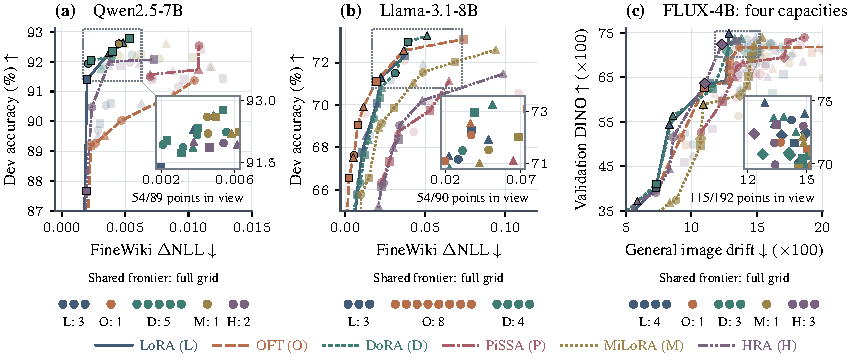
\includegraphics[width=\linewidth]{figures/peft_pareto.pdf}
\caption{Development performance--retention envelopes across LRs and capacities. Shapes denote increasing capacity: circle, square, triangle, then diamond (FLUX only). Faint points are dominated within their method. Line styles identify method frontiers. Black borders mark the shared frontier across methods. Each icon counts one configuration in the full grid (89 Qwen, 90 Llama, 192 FLUX). Insets magnify boxed regions with uniform point styling. (a,b) Dev accuracy versus FineWiki $\Delta$NLL. (c) Cat validation DINO versus general-image drift.}
\label{fig:operating-envelopes}
\end{figure}

\textbf{PiSSA frequently incurs greater retention costs.} It has the largest mean NLL increase on both coding backbones and half the mathematics settings, yet leads Llama HumanEval+. At matched LRs and capacities, PiSSA forgets most in every complete LLM comparison and constituent seed (further comparisons in Appendix~\ref{app:retention-patterns}).

PiSSA also illustrates why closer geometric preservation need not improve retention. At the largest Llama capacity, it has smaller HE and pairwise-cosine changes than LoRA (Appendix~\ref{app:hyperspherical}) but a greater NLL increase in every seed (means $\result{he_llama_pissa_forgetting}$ versus $\result{he_llama_lora_forgetting}$).

On the development frontiers, LoRA and DoRA also appear repeatedly, with DoRA reaching the highest accuracy on both backbones (\Cref{fig:operating-envelopes}a,b). OFT contributes many Llama frontier points, whereas PiSSA contributes none.

\subsection{Diffusion: recurring drift patterns, distinct retention metrics}
We next examine whether the retention patterns observed in language extend to diffusion personalization. We compare all six methods on cat personalization across parameter budgets, then extend the LoRA--OFT comparison across objects using complementary measures of retention.

\begin{table}[!htbp]
\caption{FLUX-4B test/retention scores. DINO and general drift/CLIP are $\times100$; COCO loss is unscaled. Panel (b) averages objects per seed. Shaded bold means mark the best method per budget/metric in (a), or capacity pair in (b). Budgets list rank/block sizes; HRA uses 16/32/62/124 vectors.}
\label{tab:diffusion}\label{tab:benchmark28}
\begin{center}
\textbf{(a) Cat: six methods at four approximately matched budgets}\par\smallskip
\setlength{\tabcolsep}{3pt}
\begin{tabular*}{\linewidth}{@{\extracolsep{\fill}}llcccccc}\toprule
Budget & Metric & \textcolor{LoRAColor}{LoRA} & \textcolor{OFTColor}{OFT} & \textcolor{DoRAColor}{DoRA} & \textcolor{PiSSAColor}{PiSSA} & \textcolor{MiLoRAColor}{MiLoRA} & \textcolor{HRAColor}{HRA} \\ \midrule
r4/b32 & DINO $\uparrow$ & $\result{ext_flux_flux_lora_cap4_0p0003_dino_mean}_{\pm\result{ext_flux_flux_lora_cap4_0p0003_dino_sd}}$ & $\result{ext_flux_flux_oft_cap32_0p0003_dino_mean}_{\pm\result{ext_flux_flux_oft_cap32_0p0003_dino_sd}}$ & \bestcell{DoRAColor}{$\bestmean{\result{ext_flux_flux_dora_cap4_0p0005_dino_mean}}_{\pm\result{ext_flux_flux_dora_cap4_0p0005_dino_sd}}$} & $\result{ext_flux_flux_pissa_cap4_0p0001_dino_mean}_{\pm\result{ext_flux_flux_pissa_cap4_0p0001_dino_sd}}$ & $\result{ext_flux_flux_milora_cap4_0p0001_dino_mean}_{\pm\result{ext_flux_flux_milora_cap4_0p0001_dino_sd}}$ & $\result{ext_flux_flux_hra_cap16_0p0005_dino_mean}_{\pm\result{ext_flux_flux_hra_cap16_0p0005_dino_sd}}$ \\
 & Drift $\downarrow$ & \bestcell{LoRAColor}{$\bestmean{\result{ext_flux_flux_lora_cap4_0p0003_drift_mean}}_{\pm\result{ext_flux_flux_lora_cap4_0p0003_drift_sd}}$} & $\result{ext_flux_flux_oft_cap32_0p0003_drift_mean}_{\pm\result{ext_flux_flux_oft_cap32_0p0003_drift_sd}}$ & $\result{ext_flux_flux_dora_cap4_0p0005_drift_mean}_{\pm\result{ext_flux_flux_dora_cap4_0p0005_drift_sd}}$ & $\result{ext_flux_flux_pissa_cap4_0p0001_drift_mean}_{\pm\result{ext_flux_flux_pissa_cap4_0p0001_drift_sd}}$ & $\result{ext_flux_flux_milora_cap4_0p0001_drift_mean}_{\pm\result{ext_flux_flux_milora_cap4_0p0001_drift_sd}}$ & $\result{ext_flux_flux_hra_cap16_0p0005_drift_mean}_{\pm\result{ext_flux_flux_hra_cap16_0p0005_drift_sd}}$ \\
 & CLIP $\uparrow$ & $\result{ext_flux_flux_lora_cap4_0p0003_clip_mean}_{\pm\result{ext_flux_flux_lora_cap4_0p0003_clip_sd}}$ & $\result{ext_flux_flux_oft_cap32_0p0003_clip_mean}_{\pm\result{ext_flux_flux_oft_cap32_0p0003_clip_sd}}$ & $\result{ext_flux_flux_dora_cap4_0p0005_clip_mean}_{\pm\result{ext_flux_flux_dora_cap4_0p0005_clip_sd}}$ & \bestcell{PiSSAColor}{$\bestmean{\result{ext_flux_flux_pissa_cap4_0p0001_clip_mean}}_{\pm\result{ext_flux_flux_pissa_cap4_0p0001_clip_sd}}$} & $\result{ext_flux_flux_milora_cap4_0p0001_clip_mean}_{\pm\result{ext_flux_flux_milora_cap4_0p0001_clip_sd}}$ & $\result{ext_flux_flux_hra_cap16_0p0005_clip_mean}_{\pm\result{ext_flux_flux_hra_cap16_0p0005_clip_sd}}$ \\
\addlinespace[2pt]
r8/b64 & DINO $\uparrow$ & $\result{ext_flux_flux_lora_0p0001_dino_mean}_{\pm\result{ext_flux_flux_lora_0p0001_dino_sd}}$ & $\result{ext_flux_flux_oft_5em05_dino_mean}_{\pm\result{ext_flux_flux_oft_5em05_dino_sd}}$ & $\result{ext_flux_flux_dora_0p0003_dino_mean}_{\pm\result{ext_flux_flux_dora_0p0003_dino_sd}}$ & $\result{ext_flux_flux_pissa_5em05_dino_mean}_{\pm\result{ext_flux_flux_pissa_5em05_dino_sd}}$ & $\result{ext_flux_flux_milora_5em05_dino_mean}_{\pm\result{ext_flux_flux_milora_5em05_dino_sd}}$ & \bestcell{HRAColor}{$\bestmean{\result{ext_flux_flux_hra_0p0003_dino_mean}}_{\pm\result{ext_flux_flux_hra_0p0003_dino_sd}}$} \\
 & Drift $\downarrow$ & $\result{ext_flux_flux_lora_0p0001_drift_mean}_{\pm\result{ext_flux_flux_lora_0p0001_drift_sd}}$ & $\result{ext_flux_flux_oft_5em05_drift_mean}_{\pm\result{ext_flux_flux_oft_5em05_drift_sd}}$ & $\result{ext_flux_flux_dora_0p0003_drift_mean}_{\pm\result{ext_flux_flux_dora_0p0003_drift_sd}}$ & $\result{ext_flux_flux_pissa_5em05_drift_mean}_{\pm\result{ext_flux_flux_pissa_5em05_drift_sd}}$ & $\result{ext_flux_flux_milora_5em05_drift_mean}_{\pm\result{ext_flux_flux_milora_5em05_drift_sd}}$ & \bestcell{HRAColor}{$\bestmean{\result{ext_flux_flux_hra_0p0003_drift_mean}}_{\pm\result{ext_flux_flux_hra_0p0003_drift_sd}}$} \\
 & CLIP $\uparrow$ & $\result{ext_flux_flux_lora_0p0001_clip_mean}_{\pm\result{ext_flux_flux_lora_0p0001_clip_sd}}$ & $\result{ext_flux_flux_oft_5em05_clip_mean}_{\pm\result{ext_flux_flux_oft_5em05_clip_sd}}$ & $\result{ext_flux_flux_dora_0p0003_clip_mean}_{\pm\result{ext_flux_flux_dora_0p0003_clip_sd}}$ & $\result{ext_flux_flux_pissa_5em05_clip_mean}_{\pm\result{ext_flux_flux_pissa_5em05_clip_sd}}$ & \bestcell{MiLoRAColor}{$\bestmean{\result{ext_flux_flux_milora_5em05_clip_mean}}_{\pm\result{ext_flux_flux_milora_5em05_clip_sd}}$} & $\result{ext_flux_flux_hra_0p0003_clip_mean}_{\pm\result{ext_flux_flux_hra_0p0003_clip_sd}}$ \\
\addlinespace[2pt]
r16/b128 & DINO $\uparrow$ & $\result{ext_flux_flux_lora_cap16_0p0001_dino_mean}_{\pm\result{ext_flux_flux_lora_cap16_0p0001_dino_sd}}$ & $\result{ext_flux_flux_oft_cap128_0p0001_dino_mean}_{\pm\result{ext_flux_flux_oft_cap128_0p0001_dino_sd}}$ & $\result{ext_flux_flux_dora_cap16_5em05_dino_mean}_{\pm\result{ext_flux_flux_dora_cap16_5em05_dino_sd}}$ & \bestcell{PiSSAColor}{$\bestmean{\result{ext_flux_flux_pissa_cap16_5em05_dino_mean}}_{\pm\result{ext_flux_flux_pissa_cap16_5em05_dino_sd}}$} & $\result{ext_flux_flux_milora_cap16_0p0001_dino_mean}_{\pm\result{ext_flux_flux_milora_cap16_0p0001_dino_sd}}$ & $\result{ext_flux_flux_hra_cap62_0p0005_dino_mean}_{\pm\result{ext_flux_flux_hra_cap62_0p0005_dino_sd}}$ \\
 & Drift $\downarrow$ & \bestcell{LoRAColor}{$\bestmean{\result{ext_flux_flux_lora_cap16_0p0001_drift_mean}}_{\pm\result{ext_flux_flux_lora_cap16_0p0001_drift_sd}}$} & $\result{ext_flux_flux_oft_cap128_0p0001_drift_mean}_{\pm\result{ext_flux_flux_oft_cap128_0p0001_drift_sd}}$ & $\result{ext_flux_flux_dora_cap16_5em05_drift_mean}_{\pm\result{ext_flux_flux_dora_cap16_5em05_drift_sd}}$ & $\result{ext_flux_flux_pissa_cap16_5em05_drift_mean}_{\pm\result{ext_flux_flux_pissa_cap16_5em05_drift_sd}}$ & $\result{ext_flux_flux_milora_cap16_0p0001_drift_mean}_{\pm\result{ext_flux_flux_milora_cap16_0p0001_drift_sd}}$ & $\result{ext_flux_flux_hra_cap62_0p0005_drift_mean}_{\pm\result{ext_flux_flux_hra_cap62_0p0005_drift_sd}}$ \\
 & CLIP $\uparrow$ & $\result{ext_flux_flux_lora_cap16_0p0001_clip_mean}_{\pm\result{ext_flux_flux_lora_cap16_0p0001_clip_sd}}$ & $\result{ext_flux_flux_oft_cap128_0p0001_clip_mean}_{\pm\result{ext_flux_flux_oft_cap128_0p0001_clip_sd}}$ & \bestcell{DoRAColor}{$\bestmean{\result{ext_flux_flux_dora_cap16_5em05_clip_mean}}_{\pm\result{ext_flux_flux_dora_cap16_5em05_clip_sd}}$} & $\result{ext_flux_flux_pissa_cap16_5em05_clip_mean}_{\pm\result{ext_flux_flux_pissa_cap16_5em05_clip_sd}}$ & $\result{ext_flux_flux_milora_cap16_0p0001_clip_mean}_{\pm\result{ext_flux_flux_milora_cap16_0p0001_clip_sd}}$ & $\result{ext_flux_flux_hra_cap62_0p0005_clip_mean}_{\pm\result{ext_flux_flux_hra_cap62_0p0005_clip_sd}}$ \\
\addlinespace[2pt]
r32/b256 & DINO $\uparrow$ & $\result{ext_flux_flux_lora_cap32_5em05_dino_mean}_{\pm\result{ext_flux_flux_lora_cap32_5em05_dino_sd}}$ & $\result{ext_flux_flux_oft_cap256_0p0001_dino_mean}_{\pm\result{ext_flux_flux_oft_cap256_0p0001_dino_sd}}$ & \bestcell{DoRAColor}{$\bestmean{\result{ext_flux_flux_dora_cap32_0p0001_dino_mean}}_{\pm\result{ext_flux_flux_dora_cap32_0p0001_dino_sd}}$} & $\result{ext_flux_flux_pissa_cap32_5em05_dino_mean}_{\pm\result{ext_flux_flux_pissa_cap32_5em05_dino_sd}}$ & $\result{ext_flux_flux_milora_cap32_0p0001_dino_mean}_{\pm\result{ext_flux_flux_milora_cap32_0p0001_dino_sd}}$ & $\result{ext_flux_flux_hra_cap124_0p0003_dino_mean}_{\pm\result{ext_flux_flux_hra_cap124_0p0003_dino_sd}}$ \\
 & Drift $\downarrow$ & \bestcell{LoRAColor}{$\bestmean{\result{ext_flux_flux_lora_cap32_5em05_drift_mean}}_{\pm\result{ext_flux_flux_lora_cap32_5em05_drift_sd}}$} & $\result{ext_flux_flux_oft_cap256_0p0001_drift_mean}_{\pm\result{ext_flux_flux_oft_cap256_0p0001_drift_sd}}$ & $\result{ext_flux_flux_dora_cap32_0p0001_drift_mean}_{\pm\result{ext_flux_flux_dora_cap32_0p0001_drift_sd}}$ & $\result{ext_flux_flux_pissa_cap32_5em05_drift_mean}_{\pm\result{ext_flux_flux_pissa_cap32_5em05_drift_sd}}$ & $\result{ext_flux_flux_milora_cap32_0p0001_drift_mean}_{\pm\result{ext_flux_flux_milora_cap32_0p0001_drift_sd}}$ & $\result{ext_flux_flux_hra_cap124_0p0003_drift_mean}_{\pm\result{ext_flux_flux_hra_cap124_0p0003_drift_sd}}$ \\
 & CLIP $\uparrow$ & \bestcell{LoRAColor}{$\bestmean{\result{ext_flux_flux_lora_cap32_5em05_clip_mean}}_{\pm\result{ext_flux_flux_lora_cap32_5em05_clip_sd}}$} & $\result{ext_flux_flux_oft_cap256_0p0001_clip_mean}_{\pm\result{ext_flux_flux_oft_cap256_0p0001_clip_sd}}$ & $\result{ext_flux_flux_dora_cap32_0p0001_clip_mean}_{\pm\result{ext_flux_flux_dora_cap32_0p0001_clip_sd}}$ & $\result{ext_flux_flux_pissa_cap32_5em05_clip_mean}_{\pm\result{ext_flux_flux_pissa_cap32_5em05_clip_sd}}$ & $\result{ext_flux_flux_milora_cap32_0p0001_clip_mean}_{\pm\result{ext_flux_flux_milora_cap32_0p0001_clip_sd}}$ & $\result{ext_flux_flux_hra_cap124_0p0003_clip_mean}_{\pm\result{ext_flux_flux_hra_cap124_0p0003_clip_sd}}$ \\
\bottomrule\end{tabular*}
\par\medskip\textbf{(b) 28 objects: four capacities, three LRs}\par\smallskip
\setlength{\tabcolsep}{3pt}
\begin{tabular*}{\linewidth}{@{\extracolsep{\fill}}lccccc}\toprule
Adapter & LR & Test DINO $\uparrow$ & COCO flow $\downarrow$ & General drift $\downarrow$ & General CLIP $\uparrow$\\\midrule
\loraname{} $r=4$ & $1\!\times\!10^{-4}$ & $\result{obj28_lora_4_1em04_test_mean}_{\pm\result{obj28_lora_4_1em04_test_sd}}$ & $\result{obj28_lora_4_1em04_flow_mean}_{\pm\result{obj28_lora_4_1em04_flow_sd}}$ & \bestcell{LoRAColor}{$\bestmean{\result{obj28_lora_4_1em04_drift_mean}}_{\pm\result{obj28_lora_4_1em04_drift_sd}}$} & \bestcell{LoRAColor}{$\bestmean{\result{obj28_lora_4_1em04_clip_mean}}_{\pm\result{obj28_lora_4_1em04_clip_sd}}$}\\
\loraname{} $r=8$ & $5\!\times\!10^{-5}$ & \bestcell{LoRAColor}{$\bestmean{\result{obj28_lora_8_5em05_test_mean}}_{\pm\result{obj28_lora_8_5em05_test_sd}}$} & $\result{obj28_lora_8_5em05_flow_mean}_{\pm\result{obj28_lora_8_5em05_flow_sd}}$ & \bestcell{LoRAColor}{$\bestmean{\result{obj28_lora_8_5em05_drift_mean}}_{\pm\result{obj28_lora_8_5em05_drift_sd}}$} & \bestcell{LoRAColor}{$\bestmean{\result{obj28_lora_8_5em05_clip_mean}}_{\pm\result{obj28_lora_8_5em05_clip_sd}}$}\\
\loraname{} $r=16$ & $3\!\times\!10^{-5}$ & $\result{obj28_lora_16_3em05_test_mean}_{\pm\result{obj28_lora_16_3em05_test_sd}}$ & \bestcell{LoRAColor}{$\bestmean{\result{obj28_lora_16_3em05_flow_mean}}_{\pm\result{obj28_lora_16_3em05_flow_sd}}$} & \bestcell{LoRAColor}{$\bestmean{\result{obj28_lora_16_3em05_drift_mean}}_{\pm\result{obj28_lora_16_3em05_drift_sd}}$} & \bestcell{LoRAColor}{$\bestmean{\result{obj28_lora_16_3em05_clip_mean}}_{\pm\result{obj28_lora_16_3em05_clip_sd}}$}\\
\loraname{} $r=32$ & $1\!\times\!10^{-4}$ & $\result{obj28_lora_32_1em04_test_mean}_{\pm\result{obj28_lora_32_1em04_test_sd}}$ & $\result{obj28_lora_32_1em04_flow_mean}_{\pm\result{obj28_lora_32_1em04_flow_sd}}$ & \bestcell{LoRAColor}{$\bestmean{\result{obj28_lora_32_1em04_drift_mean}}_{\pm\result{obj28_lora_32_1em04_drift_sd}}$} & \bestcell{LoRAColor}{$\bestmean{\result{obj28_lora_32_1em04_clip_mean}}_{\pm\result{obj28_lora_32_1em04_clip_sd}}$}\\
\midrule
\oftname{} $b=32$ & $1\!\times\!10^{-4}$ & \bestcell{OFTColor}{$\bestmean{\result{obj28_oft_32_1em04_test_mean}}_{\pm\result{obj28_oft_32_1em04_test_sd}}$} & \bestcell{OFTColor}{$\bestmean{\result{obj28_oft_32_1em04_flow_mean}}_{\pm\result{obj28_oft_32_1em04_flow_sd}}$} & $\result{obj28_oft_32_1em04_drift_mean}_{\pm\result{obj28_oft_32_1em04_drift_sd}}$ & $\result{obj28_oft_32_1em04_clip_mean}_{\pm\result{obj28_oft_32_1em04_clip_sd}}$\\
\oftname{} $b=64$ & $5\!\times\!10^{-5}$ & $\result{obj28_oft_64_5em05_test_mean}_{\pm\result{obj28_oft_64_5em05_test_sd}}$ & \bestcell{OFTColor}{$\bestmean{\result{obj28_oft_64_5em05_flow_mean}}_{\pm\result{obj28_oft_64_5em05_flow_sd}}$} & $\result{obj28_oft_64_5em05_drift_mean}_{\pm\result{obj28_oft_64_5em05_drift_sd}}$ & $\result{obj28_oft_64_5em05_clip_mean}_{\pm\result{obj28_oft_64_5em05_clip_sd}}$\\
\oftname{} $b=128$ & $1\!\times\!10^{-4}$ & \bestcell{OFTColor}{$\bestmean{\result{obj28_oft_128_1em04_test_mean}}_{\pm\result{obj28_oft_128_1em04_test_sd}}$} & $\result{obj28_oft_128_1em04_flow_mean}_{\pm\result{obj28_oft_128_1em04_flow_sd}}$ & $\result{obj28_oft_128_1em04_drift_mean}_{\pm\result{obj28_oft_128_1em04_drift_sd}}$ & $\result{obj28_oft_128_1em04_clip_mean}_{\pm\result{obj28_oft_128_1em04_clip_sd}}$\\
\oftname{} $b=256$ & $5\!\times\!10^{-5}$ & \bestcell{OFTColor}{$\bestmean{\result{obj28_oft_256_5em05_test_mean}}_{\pm\result{obj28_oft_256_5em05_test_sd}}$} & \bestcell{OFTColor}{$\bestmean{\result{obj28_oft_256_5em05_flow_mean}}_{\pm\result{obj28_oft_256_5em05_flow_sd}}$} & $\result{obj28_oft_256_5em05_drift_mean}_{\pm\result{obj28_oft_256_5em05_drift_sd}}$ & $\result{obj28_oft_256_5em05_clip_mean}_{\pm\result{obj28_oft_256_5em05_clip_sd}}$\\
\bottomrule\end{tabular*}

\end{center}
\end{table}


\textbf{The retention pattern recurs across cat budgets.} LoRA has the lowest mean general drift at \result{cross_cat_lora_lowest} of \result{cross_cat_selected_settings} validation-selected budgets and the second lowest at the other (\Cref{tab:diffusion}a). DoRA has higher mean test DINO than LoRA at every budget, with additional drift, and leads fidelity at the smallest and largest budgets. PiSSA exceeds LoRA's drift in all \result{cross_cat_pissa_above_lora_seeds} paired seeds; its medium-budget fidelity lead again accompanies a retention cost.

HRA has the highest mean test fidelity and lowest drift at the small budget and extends the pooled frontier, but its advantage does not persist at larger capacities. LoRA and DoRA also contribute; PiSSA contributes no frontier point (\Cref{fig:operating-envelopes}c). MiLoRA has lower mean fidelity and higher drift than LoRA at every selected budget.

Across 28 objects, LoRA and OFT have close test fidelity. LoRA has lower image drift and higher CLIP alignment at all four selected capacity pairs, while OFT has lower COCO flow loss at three (\Cref{tab:diffusion}b). These metrics distinguish preservation of generated behavior from preservation of denoising predictions at fixed noisy states.

\paragraph{Summary.}
Although task scores are often close, LoRA most consistently limits forgetting among all six methods at competitive performance. DoRA usually exceeds LoRA's mean task scores, while PiSSA often forgets more. Other methods' performance and forgetting depend on the setting. The orthogonal methods OFT and HRA offer no consistent performance--retention advantage over the four LoRA-family methods across the tested settings.
